% !TEX root = Séquence 2 - Cours - Vecteurs.tex
% Cours de la Séquence 2, copie indépendante du chapitre B1 du polycopié
% général (TeX - Polycopié et Exercices/Chapitres/Géométrie1_Vecteurs.tex),
% pour pouvoir l'adapter ici (ex. version élève à trous, comme la Séquence 1)
% sans toucher au polycopié. Recharge CLT2627.sty pour garder le rendu
% identique (boîtes Dfn/Prp/Exemple/Attention, bandeau chapitre encadré
% + puce cursive) du poly.
\documentclass[a4paper,11pt,french]{report}
% \usepackage ne peut pas prendre un chemin contenant des espaces : LaTeX
% coupe les espaces internes du nom de paquet (\zap@space, pensé pour les
% listes "pkg1, pkg2"). On charge donc CLT2627.sty par \input direct, qui
% lui n'altère pas le nom de fichier.
\input{../TeX - Polycopié et Exercices/CLT2627.sty}
\graphicspath{{../TeX - Polycopié et Exercices/}}

% Trou à compléter à la main par l'élève : espace blanc de largeur
% réglable (sans pointillés), à la place des \textcolor{red}{...} /
% \textcolor{J1}{...} du poly (réponses réservées au professeur).
\newcommand{\Trou}[1][4.5cm]{\makebox[#1][l]{}}

% Boîtes de mesure : servent à caler la hauteur d'une colonne "Exemple"
% sur celle, non connue à l'avance, de la boîte Définition posée à côté
% (voir Exemple 3 / Définition 4 ci-dessous) — même principe que
% \PropSaveBox dans "Séquence 1 - Cours - Calculs Numériques.tex", mais
% généralisé : on mesure aussi le contenu de l'Exemple lui-même, pour
% déduire l'appoint de \vspace nécessaire (DfnHeight - ExempleHeight)
% plutôt qu'une constante devinée à la main.
\newsavebox{\DfnSaveBox}
\newsavebox{\ExempleSaveBox}
\newlength{\DfnHeight}
\newlength{\ExempleHeight}

% Tableaux "Objectif / exercices" (repris de "Séquence 1 - Cours - Calculs
% Numériques.tex", mêmes macros/couleurs), placés aux endroits opportuns du
% cours pour renvoyer, pour chaque objectif déjà traité, vers les exercices
% du manuel et de la nouvelle "Séquence 2 - Feuille d'exercices - Vecteurs".
\definecolor{diffgreen}{HTML}{40C057}
\definecolor{diffblue}{HTML}{228BE6}
\definecolor{diffred}{HTML}{FA5252}
\newcommand{\starfull}[1]{{\color{#1}\ding{72}}}
\newcommand{\starempty}{{\color{gray!45}\ding{73}}}
\newcommand{\cellObj}[1]{\parbox[t]{5.2cm}{\raggedright\vspace{2pt}#1\vspace{2pt}}}
\newcommand{\cellDiff}[1]{\parbox[t]{3.6cm}{\centering\footnotesize\vspace{2pt}#1\vspace{2pt}}}
\newcommand{\headcellV}[1]{\parbox[t]{3.6cm}{\centering\vspace{2pt} \scalebox{1.1}{#1}\vspace{2pt}}}

\begin{document}
\pagestyle{empty}
% \chapter force \thispagestyle{plain} sur sa page de départ : on vide
% aussi ce style-là (défini par CLT2627.sty avec le bouton maison +
% numéro de page en pied de page), sinon \pagestyle{empty} ci-dessus ne
% suffit pas à les retirer de la première page.
\fancypagestyle{plain}{\fancyhf{}\renewcommand{\headrulewidth}{0pt}\renewcommand{\footrulewidth}{0pt}}

% Pas de \part{...} dans ce document autonome (on ne veut pas de la
% grosse page "Partie" du poly) : on fixe donc directement \thepart à
% "B" pour que le bandeau-cadre du chapitre affiche "Séquence B1" (Partie
% B - Géométrie, chapitre 1 - Vecteurs), comme dans le polycopié général.
\renewcommand{\thepart}{B}

\chapter{Notion de vecteurs}
\label{chap:vecteurs}
\begin{flushright}
\textit{\color{gray}Version compl\'et\'ee}
\end{flushright}

\section{Définition d'un vecteur}

\subsection{Translations et vecteurs}

\needspace{16\baselineskip}
\begin{minipage}{11cm}
\Dfn[Vecteur \texorpdfstring{$\Vj{AB}$}{AB}]{\par
Soient A et B deux points distincts du plan.\\
Le \textbf{vecteur} $\Vj{AB}$ est l'objet mathématique caractérisé par :
\begin{itemize}
\item[$\star$] sa \textbf{direction} : la droite (AB)
\item[$\star$] son \textbf{sens} : de A vers B
\item[$\star$] sa longueur, ou \textbf{norme}, notée $||\Vj{AB}||$ : la distance AB
\end{itemize}
L'\textbf{origine} du vecteur $\Vj{AB}$ est A et son \textbf{extrémité} est B.}
\end{minipage}
\hfill
\begin{minipage}{8cm}
\centering
\begin{tikzpicture}[x=1cm,y=1cm,>=Stealth]
\draw[-latex,thick,blue] (0,0) node[below left]{A} -- (3,1.5) node[above right]{B};
\end{tikzpicture}

\Attention{ce n'est pas pareil que le vecteur $\Vj{BA}$\\
(pas le même sens)}
\end{minipage}


\smallskip


\needspace{16\baselineskip}
\Dfn[Translation de vecteur \texorpdfstring{$\Vj{u}$}{u}]{\par
\begin{minipage}{10cm}
Soit $\Vj{u}$ un vecteur.\\
La \textbf{translation de vecteur $\Vj{u}$} est la transformation qui, à tout point A du plan, associe l'unique point A' tel que \textcolor{J1}{$\Vj{AA'} = \Vj{u}$}.
\end{minipage}
\hspace{0.5cm}
\begin{minipage}{7cm}
\centering
\begin{tikzpicture}[yscale=0.7]
    \node[left] at (1,0.7) {$\Vj{u}$};
\draw[->, line width=0.5pt] (-0.5,0)--(2.5,1) ;
\draw[-latex,thick,blue,dotted](1,-1) node[below left]{A}--(4,0) node[above right]{A'};
\end{tikzpicture}
\end{minipage}
}

\smallskip

En particulier, la translation de vecteur $\Vj{AB}$ transforme A en B (car $\Vj{AB}=\Vj{AB}$).

\needspace{18\baselineskip}
\Prp[Caractérisation par un parallélogramme]{\par
\vspace*{0.2cm}
\begin{minipage}{11cm}
Soient A, B, C, D quatre points du plan.\\
Le point D est l'image de C par la translation de vecteur $\Vj{AB}$ \fbox{si et seulement si} \textcolor{J1}{ABDC est un parallélogramme}.\\
\end{minipage}
\hfill
\begin{minipage}{7cm}
\centering
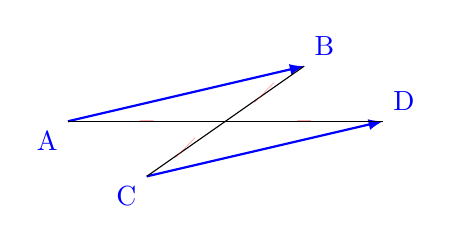
\begin{tikzpicture}[yscale=0.7]
\draw[-latex,thick,blue](0,0) node[below left]{A}--(3,1) node[above right]{B};
\draw[-latex,thick,blue](1,-1) node[below left]{C}--(4,0) node[above right]{D};
\draw (0,0)--(4,0);
\draw (1,-1)--(3,1);
\draw[red,thick] (1,0) node[scale=0.5]{|};
\draw[red,thick] (3,0) node[scale=0.5]{|};
\draw[red,thick] (1.5,-0.5) node[rotate=45,scale=0.5]{||};
\draw[red,thick] (2.5,0.5) node[rotate=45,scale=0.5]{||};
\end{tikzpicture}\\
{\tiny {\it Le parralélogramme peut être applati.}}

\end{minipage}
Cela équivaut aussi à dire que les segments [AD] et [BC] ont le \textcolor{J1}{même milieu}.

}

\medskip

\Exemple{\par
\begin{minipage}{9cm}
    Soit $ABCD$ un parallélogramme. \\
    Construire les points $E$, $F$, $G$ et $H$ tels que :
\begin{enumerate}
\item $E$ est l'image de $A$ par la translation de vecteur $\Vj{CB}$ ;
\item $F$ est l'image de $C$ par la translation de vecteur $\Vj{AB}$ ;
\item $G$ est l'image de $C$ par la translation de vecteur $\Vj{AD}$ ;
\item $H$ est l'image de $A$ par la translation de vecteur $\Vj{CD}$.
\end{enumerate}
\end{minipage}
\hfill
\begin{minipage}{8cm}
\centering
\begin{tikzpicture}[scale=0.6,x=1cm, y=1cm, >=Stealth]
    \draw[thin, gray!50] (-3,-3) grid (6,5);
    \coordinate (A) at (0,0);
    \coordinate (B) at (2,1);
    \coordinate (C) at (3,3);
    \coordinate (D) at (1,2);
    \draw[thick] (A) -- (B) -- (C) -- (D) -- cycle;
    \fill (A) circle (2pt) node[below left] {$A$};
    \fill (B) circle (2pt) node[below right] {$B$};
    \fill (C) circle (2pt) node[above right] {$C$};
    \fill (D) circle (2pt) node[above left] {$D$};
\end{tikzpicture}
\end{minipage}
}

\needspace{10\baselineskip}
\subsection{Égalité de vecteurs}

\begin{minipage}{10cm}
\Prp{\par Deux vecteurs sont {\bf égaux} s'ils ont même direction, même sens et même norme.}
\ANoter{Un vecteur n'est pas caractérisé par son origine et son extrémité : il admet une \textbf{infinité de représentants}. Autrement dit, l'origine et l'extrémité d'un vecteur ne sont pas fixes.}
\end{minipage}
\hfill
\begin{minipage}{8.5cm}
\Dfn{\par
Si $\Vj{AB}=\Vj{CD}=\Vj{EF}$, on dit que $\Vj{AB}$, $\Vj{CD}$ et $\Vj{EF}$
sont des \textbf{représentants} d'un même vecteur ($\Vj{u}$).

\begin{center}
% Vecteurs dispersés dans le plan (au lieu d'un alignement bien rangé en
% escalier) : même direction/sens/norme partout (vecteur (1,-1)), mais
% origines placées de façon plus désordonnée, pour ne pas laisser croire
% que des vecteurs égaux doivent être "rangés" les uns par rapport aux
% autres.
\begin{tikzpicture}[scale=0.65]
\draw[-latex,thick,blue] (0.4,-0.6)--(1.4,-1.6) node[midway, above right=-1pt]{$\Vj u$};
\draw[-latex,thick,blue] (0.2,1.6) node[above]{$A$}--(1.2,0.6) node[below right]{$B$};
\draw[-latex,thick,blue] (4.4,1.1) node[above]{$C$}--(5.4,0.1) node[below right]{$D$};
\draw[-latex,thick,blue] (2.6,-1.3) node[above]{$E$}--(3.6,-2.3) node[below right]{$F$};
\end{tikzpicture}
\end{center}
}
\end{minipage}

\medskip


\Exemple{
Utiliser le quadrillage pour déterminer si les égalités ci-dessous sont vraies ou fausses.
\begin{multicols}{2}
\begin{enumerate}
    \item $\Vj{AB}=\Vj{EF}$ \qquad \Trou[1.4cm]\\
    % \blue (= \color{J1} dans CLT2627.sty) remplacé par du blanc : le
    % texte reste dans la source (récupérable en repassant en \blue) mais
    % disparaît visuellement au lieu de révéler la réponse.
    \color{J1} Les vecteurs $\Vj{AB}$ et $\Vj{EF}$ ont même direction, même sens et même norme. \black
    \item $\Vj{DA}=\Vj{DB}$ \qquad \Trou[1.4cm]\\
        \color{J1} Les vecteurs $\Vj{DA}$ et $\Vj{DB}$ n'ont pas la même direction, ils ne sont donc pas égaux.
    \item $\Vj{ED}=\Vj{BD}$ \qquad \Trou[1.4cm]\\
        \color{J1} Les vecteurs $\Vj{ED}$ et $\Vj{BD}$ ont la même direction mais un sens opposé, ils ne sont donc pas égaux. \black
    \item $\Vj{AE}=\Vj{BF}$ \qquad \Trou[1.4cm]\\
    \color{J1} Les vecteurs $\Vj{AE}$ et $\Vj{BF}$ ont même direction, même sens et même norme. \black
\end{enumerate}

\begin{center}
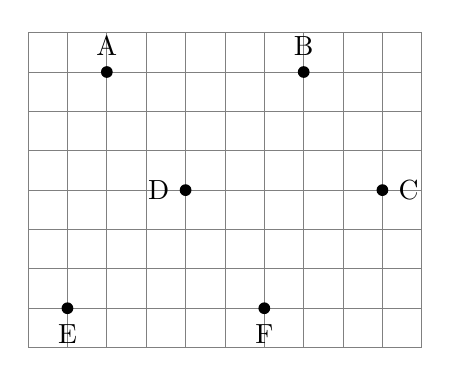
\begin{tikzpicture}[x=0.5cm, y=0.5cm]
    \draw[gray, line width=0.3pt,step=1] (0,0) grid (10,8);
    \path
        (2,7) node[circle, fill, inner sep=1.5pt, label=above: A] (A) {}
        (7,7) node[circle, fill, inner sep=1.5pt, label=above: B] (B) {}
        (9,4) node[circle, fill, inner sep=1.5pt, label=right: C] (C) {}
        (4,4) node[circle, fill, inner sep=1.5pt, label=left: D] (D) {}
        (1,1) node[circle, fill, inner sep=1.5pt, label=below:E] (E) {}
        (6,1) node[circle, fill, inner sep=1.5pt, label=below: F] (F) {};
\end{tikzpicture}
\end{center}
\end{multicols}
}

\needspace{16\baselineskip}
\subsection{Vecteurs particuliers}

% Hauteur de la colonne Exemple 3 calée sur celle de la Définition 4 :
% on mesure les deux boîtes séparément (\sbox), puis on comble l'écart
% par un \rule (largeur nulle, hauteur calculée) à l'intérieur de
% l'Exemple, plutôt qu'une constante devinée à la main. Un \vspace de fin
% de boîte serait ici une mauvaise idée : c'est de la colle, retirée par
% TeX en fin de liste verticale (donc sans effet visible), alors qu'un
% \rule occupe réellement l'espace. \refstepcounter (Dfn/Exemple) étant
% global, la mesure ci-dessous incrémenterait les compteurs "definition"
% et "exemple" une deuxième fois : on les restaure juste après chaque
% \sbox pour que la numérotation affichée plus bas reste correcte.
\edef\SaveDefinitionCounter{\arabic{definition}}%
\sbox{\DfnSaveBox}{\begin{minipage}[t]{0.58\linewidth}
\Dfn{
\begin{itemize}
\item la transformation qui laisse tous les points fixes, est appelée translation de \textbf{vecteur nul} $\Vj{0}$.\\
La norme du vecteur nul est 0 mais sa direction et son sens ne sont pas définis.
\item on appelle \textbf{vecteur opposé} au vecteur $\Vj{AB}$ le vecteur noté $-\Vj{AB}$
associé à la translation qui transforme $B$ en $A$. \\
Autrement dit, $-\Vj{AB}=\Vj{BA}$.\\
Le vecteur $-\Vj{AB}$ a donc la même direction et la même norme que $\Vj{AB}$ mais est de sens opposé.
\end{itemize}
}
\end{minipage}}%
\setlength{\DfnHeight}{\ht\DfnSaveBox}%
\addtolength{\DfnHeight}{\dp\DfnSaveBox}%
\setcounter{definition}{\SaveDefinitionCounter}%

\edef\SaveExempleCounter{\arabic{exemple}}%
\sbox{\ExempleSaveBox}{\begin{minipage}[t]{0.38\linewidth}
\Exemple{
\centering
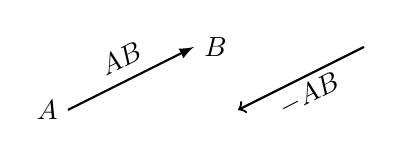
\begin{tikzpicture}[scale=0.8]
\draw[-latex,thick] (0,0) node[left]{$A$}-- (2,1) node[right]{$B$} node[midway,rotate=27,above=1pt]{$\Vj{AB}$};
\draw[<-,thick] (2.7,0) -- (4.7,1)  node[midway,rotate=27,below=-1pt]{$-\Vj{AB}$};
\end{tikzpicture}
}
\end{minipage}}%
\setlength{\ExempleHeight}{\ht\ExempleSaveBox}%
\addtolength{\ExempleHeight}{\dp\ExempleSaveBox}%
\setcounter{exemple}{\SaveExempleCounter}%

\noindent
\begin{minipage}[t]{0.58\linewidth}
\Dfn{
\begin{itemize}
\item la transformation qui laisse tous les points fixes, est appelée translation de \textbf{vecteur nul} $\Vj{0}$.\\
La norme du vecteur nul est 0 mais sa direction et son sens ne sont pas définis.
\item on appelle \textbf{vecteur opposé} au vecteur $\Vj{AB}$ le vecteur noté $-\Vj{AB}$
associé à la translation qui transforme $B$ en $A$. \\
Autrement dit, $-\Vj{AB}=\Vj{BA}$.\\
Le vecteur $-\Vj{AB}$ a donc la même direction et la même norme que $\Vj{AB}$ mais est de sens opposé.
\end{itemize}
}
\end{minipage}%
\hspace{1.2em}
\begin{minipage}[t]{0.38\linewidth}
\Exemple{
\centering
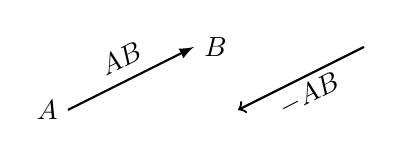
\begin{tikzpicture}[scale=0.8]
\draw[-latex,thick] (0,0) node[left]{$A$}-- (2,1) node[right]{$B$} node[midway,rotate=27,above=1pt]{$\Vj{AB}$};
\draw[<-,thick] (2.7,0) -- (4.7,1)  node[midway,rotate=27,below=-1pt]{$-\Vj{AB}$};
\end{tikzpicture}
% Réponses commentées (pourront resservir, p.ex. pour un corrigé) :
% \smallskip
% \raggedright
% \begin{itemize}
% \item \textcolor{J1}{$\Vj{AA} = \Vj{0}$} (vecteur nul)
% \item \textcolor{J1}{$-\Vj{AB} = \Vj{BA} = \Vj{CD}$} (vecteur opposé)
% \end{itemize}
\rule{0pt}{\dimexpr\DfnHeight-\ExempleHeight\relax}
}
\end{minipage}

\newpage

\subsection{Interprétation Géométrique}

\Thm{\par
\begin{minipage}{12cm}
$ABCD$ est un parallélogramme \fbox{si et seulement si} \textcolor{J1}{$\Vj{AB}$ = $\Vj{DC}$}.

\smallskip

Le parallélogramme peut-être éventuellement \og plat\fg{}.

\bigskip

\textbf{Notation : } \textcolor{J1}{on note aussi que cette égalité entraîne $\Vj{AD}=\Vj{BC}$.}
\vspace*{1.5cm}
\end{minipage}
\hspace*{1cm}
\begin{minipage}{4cm}
\begin{tikzpicture}
\draw[dashed] (1,1) -- (2,3);
\draw[dashed] (4,4) -- (3,2);
\draw[-{Stealth[length=3pt,width=2.5pt]}, line width=1.6pt] (2,3) -- (4,4);
\draw[-{Stealth[length=3pt,width=2.5pt]}, line width=1.6pt] (1,1) -- (3,2);
\node[anchor=east, font=\scriptsize] at (1,1) {A};
\node[anchor=north west, font=\scriptsize] at (3,2) {B};
\node[anchor=south east, font=\scriptsize] at (2,3) {D};
\node[anchor=south west, font=\scriptsize] at (4,4) {C};
\end{tikzpicture}
\end{minipage}
}

\bigskip

\begin{center}
{\scriptsize
\begin{tabular}{|p{5.2cm}|p{3.6cm}|p{3.6cm}|p{3.6cm}|}
\cline{2-4}
\multicolumn{1}{c|}{} & \headcellV{\starfull{diffgreen}\starempty\starempty} & \headcellV{\starempty\starfull{diffblue}\starempty} & \headcellV{\starempty\starempty\starfull{diffred}} \\
\hline
\cellObj{\textbf{Objectif 1} -- Vecteur $\Vj{MM'}$ associ\'e \`a la translation qui transforme $M$ en $M'$ ; direction, sens et norme} &
\cellDiff{Manuel - Ex~28, 30 p.185\\Feuille 2 - Ex~1, 2, 9} &
\cellDiff{Manuel - Ex~32 p.185} &
\cellDiff{} \\
\hline
\cellObj{\textbf{Objectif 2} -- \'Egalit\'e de deux vecteurs, vecteur nul} &
\cellDiff{Manuel - Ex~23, 27 p.185} &
\cellDiff{Manuel - Ex~18 p.183\\Feuille 2 - Ex~3, 4, 5, 6, 7} &
\cellDiff{} \\
\hline
\cellObj{\textbf{Objectif 3} -- Repr\'esentants d'un vecteur} &
\cellDiff{} &
\cellDiff{Manuel - Ex~31 p.185} &
\cellDiff{} \\
\hline
\cellObj{\textbf{Objectif 7} -- Caract\'erisation vectorielle du milieu d'un segment} &
\cellDiff{} &
\cellDiff{} &
\cellDiff{Feuille 2 - Ex~8} \\
\hline
\end{tabular}
}
\end{center}

\section{Somme de deux vecteurs}

\subsection{Définition et construction bout à bout}

\Dfn{
Soient $\Vj{u}$ et $\Vj{v}$ deux vecteurs. \\
La \textbf{somme} de $\Vj{u}$ et $\Vj{v}$ est le vecteur $\Vj{w}=\Vj{u}+\Vj{v}$ associé
à la translation résultant de l'enchainement des translations de vecteurs $\Vj{u}$ et de vecteur $\Vj{v}$.
}

\bigskip

\fbox{\textbf{{\large Méthode de construction bout à bout d'une somme de vecteurs.}}}

\begin{multicols}{3}
 \begin{enumerate}
 \item[] On veut construire la somme des vecteurs $\Vj{u}$ et $\Vj{v}$

 \begin{tikzpicture}[scale=0.8]
\draw[thin, gray,opacity=0.7] (0,0) grid (6,6);
\draw[-{Stealth},thick,blue] (0,0) node[left]{}--(2,1) node[above]{} node[midway,rotate=30,above]{{\large $\Vj u$}};
\draw[-{Stealth},thick,blue] (2,5)--(4,2) node[right]{} node[midway,rotate=-60,above]{{\large $\Vj v$}};
\end{tikzpicture}

\columnbreak

\item On choisit un point M quelconque
\item On construit N tel que $\Vj{MN}=\Vj{u}$.


\begin{tikzpicture}[scale=0.8]
\draw[thin, gray,opacity=0.7] (0,0) grid (6,6);
%\draw[-{Stealth},very thick,J1, dotted] (1,4) node[left]{$M$}--(3,5) node[above]{$N$} node[midway,rotate=30,above]{{\large $\Vj u$}};
\end{tikzpicture}

\columnbreak

\item On construit P tel que $\Vj{NP}=\Vj{v}$. \\
Alors $\Vj{u}+\Vj{v}=\Vj{MP}$.
\item On repère en \textcolor{red}{rouge} le vecteur somme


\begin{tikzpicture}[scale=0.8]
\draw[thin, gray,opacity=0.7] (0,0) grid (6,6);
%\draw[-{Stealth},thick,J1] (1,4) node[left]{$M$}--(3,5) node[above]{$N$} node[midway,rotate=30,above]{{\large $\Vj u$}};
%\draw[-{Stealth},thick,J1, dotted] (3,5)--(5,2) node[right]{$P$} node[midway,rotate=-60,above]{{\large $\Vj v$}};
%\draw[-{Stealth},thick,red, dashed] (1,4)--(5,2) node[midway,rotate=-25,below]{{\large $\Vj u+\Vj v$}};
\end{tikzpicture}

\end{enumerate}
\end{multicols}

\Exemple{\par
\begin{minipage}{8.5cm}
Construire le point $D$ tel que $\Vj{ED}=\Vj{BA}+\Vj{AC}$.
\begin{center}
\begin{tikzpicture}[scale=0.6]
\draw[thin, gray,opacity=0.7] (-1,0) grid (5,5);
\draw [ ] (0,2) node[above left]{A} -- ++(-3pt,-3pt) -- ++(6pt,6pt) ++(-6pt,0) -- ++(6pt,-6pt);
\draw [ ] (3,3) node[above left]{B} -- ++(-3pt,-3pt) -- ++(6pt,6pt) ++(-6pt,0) -- ++(6pt,-6pt);
\draw [ ] (1,1) node[above left]{C} -- ++(-3pt,-3pt) -- ++(6pt,6pt) ++(-6pt,0) -- ++(6pt,-6pt);
\draw [ ] (3,5) node[below right]{E} -- ++(-3pt,-3pt) -- ++(6pt,6pt) ++(-6pt,0) -- ++(6pt,-6pt);
% Construction-réponse (segments + point D) en blanc : récupérable en
% repassant "white" en "J1".
\draw[->,thick,J1] (3,5)--(0,4) ;
\draw[->,thick,J1] (0,4)--(1,3) ;
\draw [J1] (1,3) node[above right]{D} -- ++(-3pt,-3pt) -- ++(6pt,6pt) ++(-6pt,0) -- ++(6pt,-6pt);
\end{tikzpicture}
\end{center}
\end{minipage}
\hspace{1cm}
\begin{minipage}{8.5cm}
Construire le point $F$ tel que $\Vj{GF}=\Vj{AB}-\Vj{AC}$.
\begin{center}
\begin{tikzpicture}[scale=0.6]
\draw[thin, gray,opacity=0.7] (-1,0) grid (5,5);
\draw [ ] (0,2) node[above left]{A} -- ++(-3pt,-3pt) -- ++(6pt,6pt) ++(-6pt,0) -- ++(6pt,-6pt);
\draw [ ] (3,3) node[above right]{B} -- ++(-3pt,-3pt) -- ++(6pt,6pt) ++(-6pt,0) -- ++(6pt,-6pt);
\draw [ ] (1,1) node[above left]{C} -- ++(-3pt,-3pt) -- ++(6pt,6pt) ++(-6pt,0) -- ++(6pt,-6pt);
\draw [ ] (1,0) node[above left]{G} -- ++(-3pt,-3pt) -- ++(6pt,6pt) ++(-6pt,0) -- ++(6pt,-6pt);
\draw[->,thick,J1] (1,0)--(4,1) ;
\draw[->,thick,J1] (4,1)--(3,2) ;
\draw [J1] (3,2) node[above right]{F} -- ++(-3pt,-3pt) -- ++(6pt,6pt) ++(-6pt,0) -- ++(6pt,-6pt);
\end{tikzpicture}
\end{center}
\end{minipage}
}

\needspace{10\baselineskip}
\subsection{Relation de Chasles}

\Prp[Relation de Chasles]{\par
\begin{minipage}{10cm}
Soient $A$ et $B$ deux points du plan. Pour tout point $M$, on a :
$$
\Vj{AB}=\Vj{AM}+\Vj{MB}.
$$
\vspace*{1cm}
Aller d'Argentan à B puis de B à Coutances, c'est, finalement, aller d'Argentan à Coutances.
\end{minipage}
\hspace{3cm}
\begin{minipage}{5cm}
\begin{tikzpicture}
\draw [ ] (0,0) node[above left]{A} -- ++(-3pt,-3pt) -- ++(6pt,6pt) ++(-6pt,0) -- ++(6pt,-6pt);
\draw [ ] (4,2) node[above left]{B} -- ++(-3pt,-3pt) -- ++(6pt,6pt) ++(-6pt,0) -- ++(6pt,-6pt);
\end{tikzpicture}
\end{minipage}
}

\needspace{12\baselineskip}
\Exemple{
Simplifier les expressions en utilisant la relation de Chasles :
\begin{enumerate}
\item$\Vj{AB}-\Vj{AC}-\Vj{CB}$\\
\textcolor{J1}{$\Vj{AB}-\Vj{AC}-\Vj{CB} = \Vj{AB}-(\Vj{AC}+\Vj{CB}) = \Vj{AB}-\Vj{AB} = \Vj{0}$.}
\medskip
\item$\Vj{BC}-\Vj{BA}+\Vj{BD}-\Vj{BC}$\\
\textcolor{J1}{$\Vj{BC}-\Vj{BA}+\Vj{BD}-\Vj{BC} = \Vj{BD}-\Vj{BA} = \Vj{AD}$.}
\end{enumerate}
}

\bigskip

\begin{center}
{\scriptsize
\begin{tabular}{|p{5.2cm}|p{3.6cm}|p{3.6cm}|p{3.6cm}|}
\cline{2-4}
\multicolumn{1}{c|}{} & \headcellV{\starfull{diffgreen}\starempty\starempty} & \headcellV{\starempty\starfull{diffblue}\starempty} & \headcellV{\starempty\starempty\starfull{diffred}} \\
\hline
\cellObj{\textbf{Objectif 4} -- Somme de deux vecteurs et relation de Chasles} &
\cellDiff{Manuel - Ex~39 p.186,\\42 p.187\\Feuille 2 - Ex~11} &
\cellDiff{Manuel - Ex~33, 35, 38 p.185-186,\\43, 45 p.187, 72 p.192\\Feuille 2 - Ex~10, 12} &
\cellDiff{} \\
\hline
\end{tabular}
}
\end{center}

\needspace{10\baselineskip}
\section{Multiplication par un scalaire}

\needspace{20\baselineskip}
\Exemple[introductif]{
Intéressons-nous tout d'abord à deux exemples : \\
\begin{minipage}{8cm}
\begin{enumerate}
	\item $\Vj{u}$ est le vecteur
			\begin{itemize}
				\item de même direction que $\Vj{v}$ ;
				\item de même sens que $\Vj{v}$ ;
				\item de norme $3$ fois de celle de $\Vj{v}$.
			\end{itemize}
			On écrit alors : \textcolor{J1}{$\Vj{u} = 3\Vj{v}$}
	\item $\Vj{j}$ est le vecteur
			\begin{itemize}
				\item de même direction que $\Vj{i}$ ;
				\item de sens opposé à $\Vj{i}$ ;
				\item de norme deux fois celle de $\Vj{i}$.
			\end{itemize}
			On écrit alors : \textcolor{J1}{$\Vj{j} = -2\Vj{i}$}
\end{enumerate}
\end{minipage}
\hspace{3cm}
\begin{minipage}{8cm}
\begin{tikzpicture}[scale=0.5]
\draw[thin,gray,opacity=0.7] (0,0) grid  (12,12);
\draw[->,ultra thick] (3,5)--(1,7) node[midway,rotate=-45,above]{$\Vj v$};
\draw[->,ultra thick,J1] (7,5)--(1,11) node[midway,rotate=-45,above]{$\Vj u$};
\draw[->,ultra thick] (7,9)--(9,11) node[midway,rotate=45,above]{$\Vj i$};
\draw[->,ultra thick,J1] (11,5)--(7,1) node[midway,rotate=45,above]{$\Vj j$};
\end{tikzpicture}
\end{minipage}
}

\needspace{10\baselineskip}
\Dfn[Produit d'un vecteur par un nombre réel]{
Soit $\Vj{u}$ un vecteur non nul et soit $k$ un réel non nul. Alors le vecteur {\Large $\Vj{v}= \textcolor{red}{k}\Vj{u}$} est :
\begin{center}
\begin{tabular}{|p{5cm}|p{5cm}|}
\hline
\centering si $\textcolor{red}{k}>0$ & \centering si $\textcolor{red}{k}<0$\cr
\hline
de même direction que $\Vj{u}$  & de même direction que $\Vj{u}$ \\
de même sens que $\Vj{u}$ & de sens inverse de $\Vj{u}$\\
de norme $k$ fois celle de $\Vj{u}$ & de norme $(-k)$ fois celle de $\Vj{u}$\\
\hline
\end{tabular}
\end{center}
}

\needspace{20\baselineskip}
\Exemple{

\begin{enumerate}
\item Exprimer le vecteur $\Vj{AC}$ en fonction du vecteur $\Vj{AB}$ dans chacun des cas suivants :
\\[0.5em]
\begin{tabular}{p{0.5\textwidth} p{0.5\textwidth}}
\begin{tikzpicture}[x=1.5cm, y=1cm, >=stealth]
    \draw[->] (-0.5,0) -- (2.5,0);
    \foreach \x in {-0.5,0,...,2.5} {
        \draw (\x, 0.08) -- (\x, -0.08);
    }
    \fill (0,0) circle (2pt) node[above=2pt] {$A$};
    \fill (1,0) circle (2pt) node[above=2pt] {$B$};
    \fill (2,0) circle (2pt) node[above=2pt] {$C$};
    \node at (1,-0.6) {\textcolor{J1}{$\Vj{AC}=2\Vj{AB}$}};
\end{tikzpicture}
&
\begin{tikzpicture}[x=1.5cm, y=1cm, >=stealth]
    \draw[->] (-2,0) -- (2,0);
    \foreach \x in {-2,-1.5,...,2} {
        \draw (\x, 0.08) -- (\x, -0.08);
    }
    \fill (1,0) circle (2pt) node[above=2pt] {$A$};
    \fill (1.5,0) circle (2pt) node[above=2pt] {$B$};
    \fill (-1.5,0) circle (2pt) node[above=2pt] {$C$};
    \node at (0,-0.6) {\textcolor{J1}{$\Vj{AC}=-5\Vj{AB}$}};
\end{tikzpicture}
\end{tabular}

\medskip

\item Dans chacun des cas suivants, représenter le vecteur $\Vj{AC}$ tel que :
\\[0.5em]
\begin{tabular}{p{0.5\textwidth} p{0.5\textwidth}}
 $\Vj{AC} = -3\Vj{AB}$ & $\Vj{AC} = \dfrac{1}{3}\Vj{AB}$ \\[1em]
\begin{tikzpicture}[x=1.2cm, y=1cm, >=stealth]
    \draw[->] (-2,0) -- (2.5,0);
    \foreach \x in {-2,-1.5,...,2.5} {
        \draw (\x, 0.08) -- (\x, -0.08);
    }
    \fill (0,0) circle (2pt) node[above=2pt] {$A$};
    \fill (0.5,0) circle (2pt) node[above=2pt] {$B$};
    \fill[J1] (-1.5,0) circle (2pt) node[above=2pt] {\textcolor{J1}{$C$}};
\end{tikzpicture}
&
\begin{tikzpicture}[x=1.2cm, y=1cm, >=stealth]
    \draw[->] (-1.5,0) -- (2.5,0);
    \foreach \x in {-1.5,-1,...,2.5} {
        \draw (\x, 0.08) -- (\x, -0.08);
    }
    \fill (0,0) circle (2pt) node[above=2pt] {$A$};
    \fill (1.5,0) circle (2pt) node[above=2pt] {$B$};
    \fill[J1] (0.5,0) circle (2pt) node[above=2pt] {\textcolor{J1}{$C$}};
\end{tikzpicture}
\end{tabular}

\medskip

\item Construire dans la figure ci-dessous des représentants des vecteurs $2\Vj{u}$, $-\Vj{u}$ et $\dfrac12\Vj{u}$ :

\begin{center}
\begin{tikzpicture}
\draw[thin,gray,opacity=0.7] (-3,-1) grid (6,3);
\draw[->,thick,blue] (0,0) -- (3,1) node[midway,rotate=20,above]{$\Vj{u}$};
\draw[->,thick,J1] (-2,-1) -- (4,1) node[midway,rotate=20,above]{$2\Vj{u}$};
\draw[->,thick,J1] (2,3) -- (-1,2) node[midway,rotate=20,above]{$-\Vj{u}$};
\draw[->,thick,J1] (-3,2) -- (-1.5,2.5) node[midway,rotate=20,above]{$\frac12\Vj{u}$};
\end{tikzpicture}
\end{center}

\end{enumerate}
}

\section{Vecteurs colinéaires}

\needspace{16\baselineskip}
\noindent
\begin{minipage}[t]{0.55\linewidth}
\Dfn[Vecteurs colinéaires]{par
Deux vecteurs $\Vj{u}$ et $\Vj{v}$ sont dit \textbf{colinéaires} s'il existe un réel $k$ tel que $\Vj{v}=k\Vj{u}$ ou $\Vj{u}=k\Vj{v}$.
}
\ANoter{
\begin{itemize}
\item deux vecteurs sont colinéaires si et seulement s'ils ont \textbf{même direction}.
\item le vecteur nul est colinéaire à n'importe quel vecteur. En effet, $\Vj{0}=0\Vj{u}$.
\end{itemize}
}

\end{minipage}%
\hspace{1.2em}
\begin{minipage}[t]{0.40\linewidth}
\Exemple{\par
\centering
\begin{tikzpicture}[scale=0.65]
\draw[thin,gray,opacity=0.5] (0,0) grid (6,4);
\draw[->,thick,blue] (0.5,0.5) -- (1.5,1) node[midway,rotate=27,above]{$\Vj u$};
\draw[->,thick,J1] (5,3) -- (3,2) node[midway,rotate=27,above]{$\Vj v$};
\end{tikzpicture}

\smallskip
\raggedright
\textcolor{J1}{$\Vj{v} = -2\Vj{u}$}\\
%, donc $\Vj{u}$ et $\Vj{v}$ sont colinéaires.
}
\end{minipage}

\medskip

\medskip

\ANoter[À retenir]{la notion de colinéarité est fortement liée à celle de parallélisme et d'alignement.}

\needspace{20\baselineskip}
\Prp[Colinéarité et parallélisme]{
\begin{spacing}{1.7}
Soient A, B, C et D quatre points.

\medskip

Les vecteurs $\Vj{AB}$ et $\Vj{CD}$ sont colinéaires si et seulement si les droites (AB) et (CD) sont \textcolor{J1}{parallèles (ou confondues)}.
\end{spacing}
\hspace{1cm}
\begin{minipage}{6cm}
\begin{tikzpicture}[scale=0.7]
\draw[thin,gray,opacity=0.5] (0,0) grid (8,5);
\draw[|-{Stealth[length=10pt,inset=2pt]},very thick,airforceblue] (1,2) node[below=2pt]{A} --(2,4) node[above=2pt]{B} node[midway,rotate=60,above=2pt]{$\Vj{AB}$};
\draw[dotted,red, thick](0,0) -- (1,2);
\draw[dotted,red, thick](2,4) --(2.5,5) ;
\draw[|-{Stealth[length=10pt,inset=2pt]},very thick,airforceblue] (6,5) node[below right]{C} --(4,1) node[below=2pt]{D} node[midway,rotate=60,above=2pt]{$\Vj{CD}$};
\draw[dotted,red](3.5,0) -- (4,1);
\end{tikzpicture}
\end{minipage}
\hspace{0.5cm}
\begin{minipage}{12cm}
\textbf{Rédaction : }

\vspace*{1cm}

Ici, on a : $\Vj{CD} = \textcolor{J1}{-2} \  \Vj{AB}$ donc $\Vj{AB}$ et $\Vj{CD}$ sont \textcolor{J1}{colinéaires}.

\medskip

Ainsi : les droites \textcolor{J1}{$(AB)$} et \textcolor{J1}{$(CD)$} sont \textcolor{J1}{parallèles}.
\end{minipage}
}

\needspace{12\baselineskip}
\Prp[Colinéarité et alignement]{
\begin{spacing}{1.7}
Soient A, B et C trois points distincts.

\medskip

Les points A, B et C sont alignés si et seulement si les vecteurs $\Vj{AB}$ et $\Vj{AC}$ sont \textcolor{J1}{colinéaires}.
\end{spacing}

\medskip

\begin{minipage}{10cm}
\textbf{Notation : }

\vspace*{1cm}

Ici, on a : $\Vj{AB} = \dfrac35 \  \Vj{AC}$ donc \textcolor{J1}{$\Vj{AB}$} et \textcolor{J1}{$\Vj{AC}$} sont \textcolor{J1}{colinéaires}.

\medskip

Ainsi : \textcolor{J1}{les points A, B et C sont alignés.}
\end{minipage}
\hspace{1cm}
\begin{minipage}{6cm}
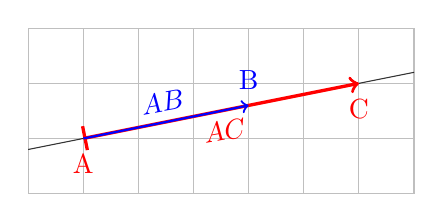
\begin{tikzpicture}[scale=0.7]
\draw[thin,gray,opacity=0.5] (0,1) grid (7,4);
\draw[opacity=0.8](0,1.8) --(7,3.2) ;
\draw[|->,very thick,red] (1,2) node[below=2pt]{A} --(6,3) node[below=2pt]{C} node[midway,rotate=10,below]{$\Vj{AC}$};
\draw[->, thick,blue] (1,2) --(4,2.6) node[above=2pt]{B} node[midway,rotate=10,above]{$\Vj{AB}$};
\end{tikzpicture}
\end{minipage}
}

\bigskip

\begin{center}
{\scriptsize
\begin{tabular}{|p{5.2cm}|p{3.6cm}|p{3.6cm}|p{3.6cm}|}
\cline{2-4}
\multicolumn{1}{c|}{} & \headcellV{\starfull{diffgreen}\starempty\starempty} & \headcellV{\starempty\starfull{diffblue}\starempty} & \headcellV{\starempty\starempty\starfull{diffred}} \\
\hline
\cellObj{\textbf{Objectif 5} -- Produit d'un vecteur par un nombre r\'eel et colin\'earit\'e de deux vecteurs} &
\cellDiff{Manuel - Ex~19 p.207,\\42, 44 p.208-210, 61 p.210} &
\cellDiff{Manuel - Ex~41 p.208-210,\\74 p.212\\Feuille 2 - Ex~13, 14, 15} &
\cellDiff{Manuel - Ex~45 p.208-210,\\75 p.212} \\
\hline
\cellObj{\textbf{Objectif 6} -- D\'ecomposition d'un vecteur en fonction de deux vecteurs non colin\'eaires} &
\cellDiff{} &
\cellDiff{} &
\cellDiff{Feuille 2 - Ex~16} \\
\hline
\end{tabular}
}
\end{center}

\end{document}
